\documentclass[border=3pt]{standalone}
% Preâmbulo compartilhado pelos diagramas TikZ da aula 7 de IHR (Emoção)
\usepackage[T1]{fontenc}
\usepackage[utf8]{inputenc}
\usepackage{lmodern}
\usepackage{amsmath}
\usepackage{xcolor}
\usepackage{tikz}
\usetikzlibrary{arrows.meta,angles,quotes,decorations.pathmorphing,decorations.pathreplacing,calc,
                positioning,shapes.geometric,shapes.misc,backgrounds,fit,
                math}

% Paleta (mesma dos SVGs originais)
% Paleta da disciplina de IHR: acento azul (#1A6FB5), cor de destaque do tema.
% (o nome "dblue" é mantido para não alterar todos os diagramas)
\definecolor{dblue}{HTML}{1A6FB5}
\definecolor{dorange}{HTML}{B3541E}
\definecolor{dgreen}{HTML}{4A7C59}
\definecolor{dred}{HTML}{9C4B4B}
\definecolor{dcream}{HTML}{F4F1EA}
\definecolor{dshade}{HTML}{DDD7C9}

% Função gaussiana (não normalizada por padrão de escala visual)
\pgfmathdeclarefunction{gauss}{3}{%
  \pgfmathparse{1/(#3*sqrt(2*pi))*exp(-((#1-#2)^2)/(2*#3^2))}%
}

% Estilos comuns (prefixo d... para não colidir com chaves internas do pgf)
\tikzset{
  >={Stealth[length=2mm]},
  dguide/.style={gray!55, dashed, line width=0.4pt},
  daxis/.style={gray!60, line width=0.7pt, ->},
  dbody/.style={fill=black!3, draw=black!80, line width=1pt},
  dacc/.style={draw=dblue, line width=1pt},
  dlbl/.style={black!55, font=\small},
  dsub/.style={black!45, font=\footnotesize},
  dstate/.style={circle, draw=black!80, fill=dcream, line width=1pt,
                 minimum size=17mm, font=\large, inner sep=1pt},
  dobs/.style={circle, draw=black!80, fill=dshade, line width=1pt,
               minimum size=14mm, font=\large, inner sep=1pt},
  dbox/.style={rounded corners=2pt, draw=black!80, fill=dcream, line width=1pt,
               align=center, inner sep=6pt},
  dop/.style={circle, draw=black!80, fill=white, line width=1pt,
              minimum size=6mm, inner sep=0pt, font=\small},
  dtrans/.style={->, dblue, line width=1pt},
  dmeas/.style={->, dorange, line width=1pt},
  dcurve/.style={line width=1pt, dblue},
  dcurveb/.style={line width=1.4pt, dorange},
}

\begin{document}
\hyphenpenalty=10000 \exhyphenpenalty=10000 \tolerance=9999 \emergencystretch=3em
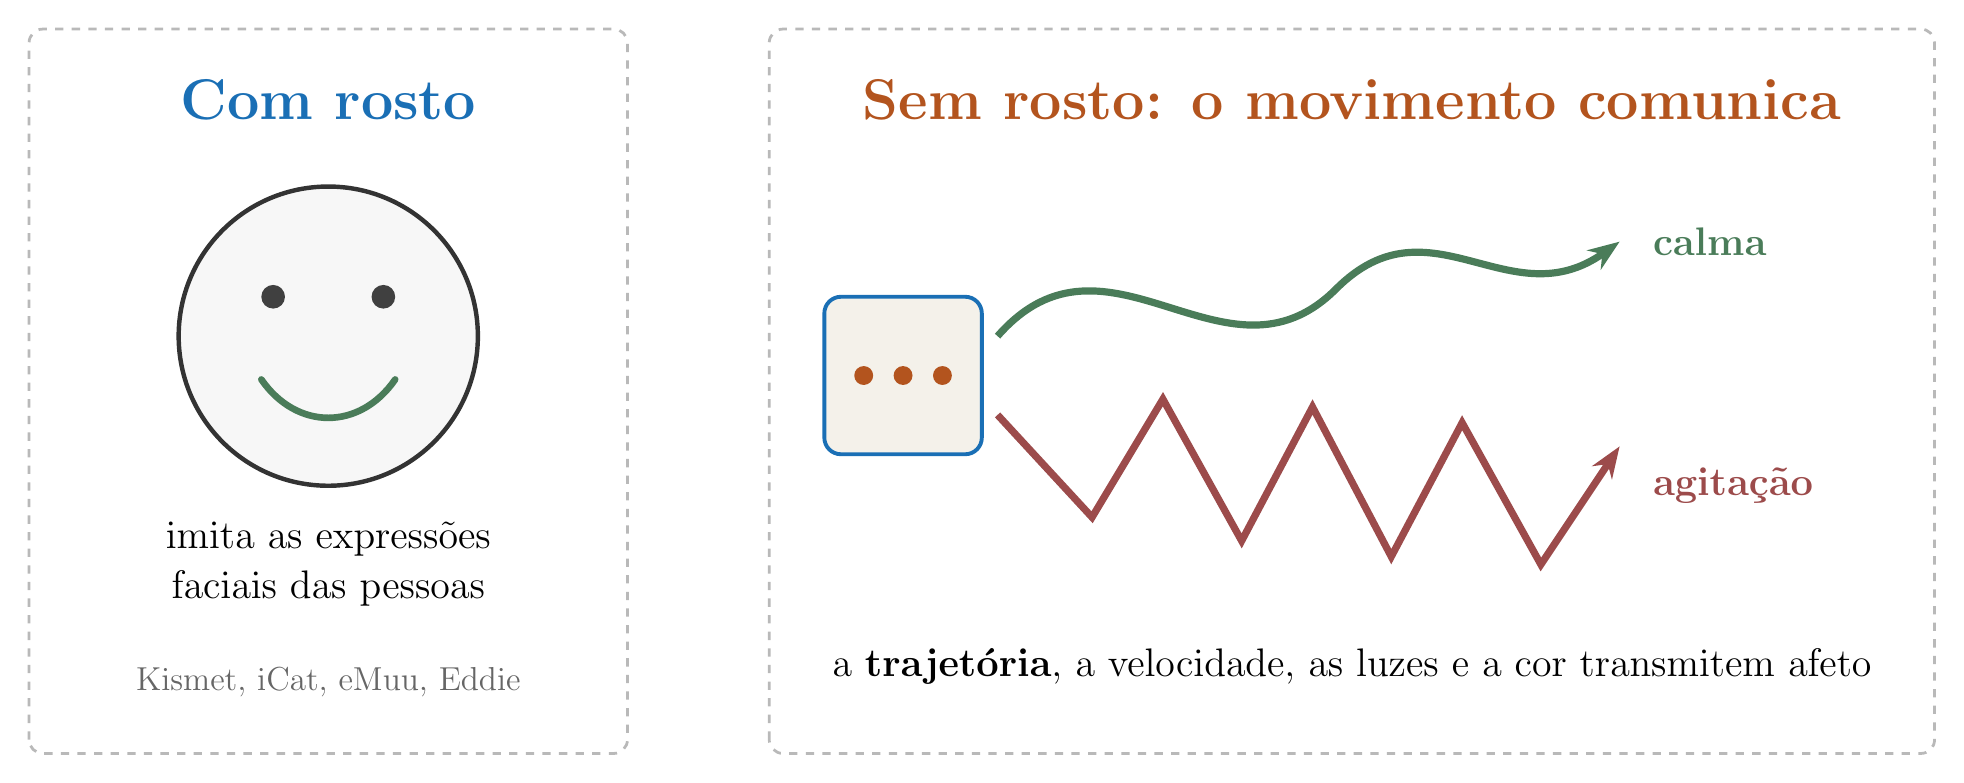
\begin{tikzpicture}[x=1cm,y=1cm]

  % ================= Com rosto =================
  \begin{scope}[shift={(0,0)}]
    \draw[dguide, rounded corners=5pt, line width=1pt] (-3.8,-4.3) rectangle (3.8,4.9);
    \node[font=\huge\bfseries, dblue] at (0,4.0) {Com rosto};
    \draw[dbody, line width=1.6pt] (0,1.0) circle (1.9);
    \fill[black!75] (-0.7,1.5) circle (0.15) (0.7,1.5) circle (0.15);
    \draw[dgreen, line width=2.4pt, line cap=round] (-0.85,0.45) .. controls (-0.4,-0.2) and (0.4,-0.2) .. (0.85,0.45);
    \node[font=\Large, align=center, text width=7.0cm] at (0,-1.9) {imita as expressões faciais das pessoas};
    \node[font=\large, black!60, align=center, text width=7.0cm] at (0,-3.4) {Kismet, iCat, eMuu, Eddie};
  \end{scope}

  % ================= Sem rosto =================
  \begin{scope}[shift={(9.4,0)}]
    \draw[dguide, rounded corners=5pt, line width=1pt] (-3.8,-4.3) rectangle (11.0,4.9);
    \node[font=\huge\bfseries, dorange] at (3.6,4.0) {Sem rosto: o movimento comunica};
    % robô (vista de cima)
    \draw[line width=1.4pt, draw=dblue, fill=dcream, rounded corners=6pt] (-3.1,-0.5) rectangle (-1.1,1.5);
    \fill[dorange] (-2.6,0.5) circle (0.12) (-2.1,0.5) circle (0.12) (-1.6,0.5) circle (0.12);
    % trajetória suave
    \draw[dgreen, line width=2.6pt, -{Stealth[length=4mm]}] (-0.9,1.0) .. controls (0.5,2.6) and (2.0,0.2) .. (3.4,1.6) .. controls (4.6,2.8) and (5.6,1.2) .. (7.0,2.2);
    \node[font=\Large\bfseries, dgreen, align=center, anchor=west] at (7.3,2.2) {calma};
    % trajetória brusca
    \draw[dred, line width=2.6pt, -{Stealth[length=4mm]}] (-0.9,0.0) -- (0.3,-1.3) -- (1.2,0.2) -- (2.2,-1.6) -- (3.1,0.1) -- (4.1,-1.8) -- (5.0,-0.1) -- (6.0,-1.9) -- (7.0,-0.4);
    \node[font=\Large\bfseries, dred, align=center, anchor=west] at (7.3,-0.9) {agitação};
    \node[font=\Large, align=center, text width=13.5cm] at (3.6,-3.2) {a \textbf{trajetória}, a velocidade, as luzes e a cor transmitem afeto};
  \end{scope}

\end{tikzpicture}
\end{document}
